\chapter{INTRODUCTION}
\label{ch1}

\section{Origins of Computational Chemistry}
The seeds of computational chemistry were sown in the mid-1800s with Ludwig
Eduard Boltzmann's formulation of \emph{statistical mechanics}. In an era when
the existence of atoms and molecules was hotly disputed within the physics
community, Boltzmann fathered a theory in which the behavior and interaction of
individual atoms or molecules on the microscopic scale could be used to
describe and predict macroscopic phenomena. Using his theorems and equations,
it became possible to reduce the problem of simulating $\sim 10^{23}$ molecules
to simulating $\sim 1$ molecule. Boltzmann used this to great effect in
describing and deriving previously-known, phenomenological equations for ideal
gases, such as the widely known equation of state, $P V = n R T$. All that
remains to provide the foundation for using molecular simulations is the proper
description of atoms and molecules on the microscopic scale.

The theories required to accurately model the behavior of individual atoms
interacting with each other and their surroundings would not be developed until
the first half of the $20^{th}$ century with the advent of \textit{quantum
mechanics}. The limits of classical mechanics became apparent when considering
the Rayleigh-Jeans formula for calculating the spectral emission of a radiating
black body. The Rayleigh-Jeans law, given by Eq. \ref{eq1:RayleighJeans}, is
completely derived using the laws of classical mechanics. By looking at Eq.
\ref{eq1:RayleighJeans}, we see that the emission spectrum diverges at high
frequencies ($\nu$)---a clear violation of the well-established law of
conservation of energy.
\begin{equation}
   B_{\nu} (T)  = \frac{2 \nu^2 k T} {c^2}
   \label{eq1:RayleighJeans}
\end{equation}
To address this apparent disparity, Max Planck suggested that the error in the
classical mechanical approach was to assume a continuous emission spectrum.
Instead, Planck suggested that the emission spectra was quantized, leading to an
equation that agreed much closer with experiment. This idea of quantized energy
emissions, while developed to reconcile the mathematics of black-body radiation
with experimental measurements, would forever change our understanding of the
microscopic world.

As quantum mechanics matured, our ability to explain and predict behavior at the
atomic scale dramatically improved. In 1929, Paul Dirac proclaimed, ``The
fundamental laws necessary for the mathematical treatment of a large part of
physics and the whole of chemistry are thus completely known, and the difficulty
lies only in the fact that the application of these laws leads to equations that
are too complex to be solved.'' Even approximations designed to simplify the
equations of quantum mechanics in molecular systems resulted in computations too
complex to apply to all but the simplest systems. With the fundamental theory
necessary to describe single molecules and the machinery required to extend
that description to experimental measurements at our disposal, computers
provided the catalyst that thrusted theoretical chemistry into a prominent role
in chemical research.

The next sections will describe the theory of quantum mechanics and the
approximations typically employed to simplify its equations, followed by
a description of statistical mechanics.

\subsection{Quantum Mechanics}

Twenty years after Planck introduced the idea of quantized oscillators to
explain black-body radiation, Erwin Schr\"odinger introduced a wave equation
formulation of quantum mechanics (QM). \cite{Schrodinger1926} Schr\"odinger's
equation (Eq. \ref{eq1:SchrodingerEquation}) bears a strong resemblance to
Hamilton's formulation of classical mechanics by employing an analogous
\textit{Hamiltonian} operator comprised of a kinetic energy term (related to the
momentum operator) and a potential energy term.
\begin{align}
   E \Psi(\vec{x}, t) & = \hat{H} \Psi(\vec{x}) \nonumber \\
   & = \left ( -\frac {\hbar ^ 2} {2 m} \bigtriangledown ^ 2 + V(\vec{x})
   \right) \Psi(\vec{x})
   \label{eq1:SchrodingerEquation}
\end{align}
In Eq. \ref{eq1:SchrodingerEquation}, $E$ is the total energy, $\hat{H}$ is the
Hamiltonian operator, and $\Psi(\vec{x}, t)$ is the wavefunction---the central
object of Schr\"odinger's equation containing all of the information and
properties inherent to the system.

Eq. \ref{eq1:SchrodingerEquation} is a special form of Schr\"odinger's
equation corresponding to a stationary state (\ie the potential function is
time-independent, so the energy for that state is constant). In chemistry when
we wish to calculate observable properties of a system composed of atoms, the
kinetic energy is the sum of the kinetic energies of the atomic particles in the
system, and the potential energy is calculated as the interaction of all charged
particles---protons and electrons---in the electric field they create (plus any
external field that may be present).

The wavefunction contains all of the information about each of the particles in
the system. As the number of particles in the system increases, so too does the
complexity of the wavefunction and the effort required to solve Eq.
\ref{eq1:SchrodingerEquation}. Therefore, we turn to a number of approximations
developed to simplify computing a solution to Schr\"odinger's equation.

\subsubsection{Born-Oppenheimer Approximation}

The Born-Oppenheimer approximation (BOA) is pervasive in the field of
computational chemistry. Electrons can move far more rapidly than nucleons since
electrons are roughly 1000 times lighter. This implies that electrons can
reorganize around moving nuclei so quickly that nuclear protons are always
subject to the potential from the average electric field generated by the
electrons.

Using the BOA, the wavefunction of a molecular system can be separated into two
parts: an electronic part where the nuclei are treated as fixed point charges,
and a nuclear part where the nuclei move through the average electric field
generated by the electrons.  \cite{McQuarrie_Book_PhysChem_1997} So critical is
the BOA to computational chemistry that it appears at the heart of nearly every
computational molecular model.

\subsubsection{Computational Quantum Mechanics}
\label{sec1:CompQuantumMech}

The main goal of most QM calculations in chemistry and molecular physics is to
determine atomic and molecular properties of the system by estimating the
electronic part of the wavefunction from the BOA. These calculations have
provided valuable assistance to experimental investigations. QM calculations
can provide reliable measurements of molecular geometries,
\cite{Jeletic_JOrganometChem_2011_v696_p3127} potential and free energy barriers
of chemical reactions, \cite{Chandrasekhar_JAmChemSoc_1985_v107_p154} ionization
energies, \cite{Watson_ChemPhysLett_2013_v555_p235} proton affinities and
gas-phase basicities \cite{Range_PhysChemChemPhys_2005_v7_p3070}, and many other
chemical and molecular properties. \cite{Hehre_Ab_inito_MO_Theory_Book_1986}

These calculations are becoming routine as more and more experimental studies
employ some form of calculation to help interpret results or strengthen
conclusions. Despite all their successes and the rapid increase of computational
power over recent years, however, the computational demands of QM methods often
remain prohibitively high for systems with more than 100 -- 200 atoms.
Furthermore for researchers interested in these large systems, calculations on a
single arrangement of atomic nuclei becomes increasingly insufficient to
quantify the behavior of those systems.

For such applications, we turn our attention back to statistical mechanics with
the aim of ultimately applying those principles to molecular mechanical
simulations of large molecules that often contain thousands---even hundreds of
thousands---of atoms.

\subsection{Statistical Mechanics}

Macroscopic chemical systems are composed of a vast number of atoms---on the
order of Avogadro's number, or $6.022 \times 10 ^ {23}$. How, then, can our
calculations of a single molecule or a small cluster of molecules be used to
predict the behavior of a collection of $10 ^ {23}$ molecules? For that we turn
to statistical mechanics and the idea of an \emph{ensemble}.

In a system with $N$ particles (where $N$ is typically on the order of
Avagadro's number in magnitude), there are $6 N$ total degrees of freedom in the
system corresponding to the position and momentum of each particle in all three
dimensions. This ultra-high, $6N$-dimensional space is referred to as
\emph{phase space}, and the collection of all points that conform to a small set
of thermodynamic constraints---\eg constant volume or energy---represents an
ensemble. \cite{McQuarrie_Book_StatMech_1973} The connection between this
imaginary ensemble of systems and experimental measurements of real systems was
provided by Josiah Gibbs. The experimental value of any system in the lab is
postulated to be equal to the value of that mechanical observable averaged over
every member of the ensemble. \cite{McQuarrie_Book_StatMech_1973} By knowing the
probability of finding a member of an ensemble with a given set of properties,
this ensemble average can be calculated according to Eq. \ref{eq1:EnsembleAvg}.

\begin{align}
   \left < A \right > & = \frac {\sum_a W(a) A(a)} {\sum_a W(a)} \nonumber \\
                      & = \sum_a P(a) A(a)
   \label{eq1:EnsembleAvg}
\end{align}
$W(a)$ in Eq. \ref{eq1:EnsembleAvg} can be thought of as the number of states in
the ensemble with the same value of $A$. $P(a)$ is the normalized probability
for that state, where $\sum_a W(a)$ is the normalization factor.

Given that there are on the order of $10^{23}$ particles in the typical system,
the number of ensemble members from which the average is calculated appears at
first glance to be intractable. However, it turns out that the mean square
fluctuations of measurable properties within the ensemble scale as roughly $1 /
\sqrt{N}$ where $N$ is the number of particles in the system.  Because $N$ is on
the order of $10 ^ {23}$, the fluctuations around the most probable value in the
ensemble vanish and the ensemble average and most probable value become
identical. The problem of calculating the ensemble average of a desired property
is reduced to the far more tractable task of calculating its most probable
value.

The most commonly used ensemble, called the \emph{canonical} ensemble, is
constrained such that each member has the same number of particles, volume, and
temperature (NVT). Other common ensembles include the microcanonical ensemble
(NVE), the grand canonical ensemble ($\mu$VT), and the isobaric-isothermal
ensemble (NpT), where E, $\mu$, and p stand for constant energy, chemical
potential, and pressure, respectively. At typical temperatures and particle
densities, the fluctuations of mechanical properties in each of these ensembles
becomes negligible. Therefore, these ensembles are effectively equivalent to one
another, allowing us to choose the one that is most convenient to work with
mathematically.

The link between these ensembles and thermodynamics is the natural logarithm of
the \emph{partition function}, which happens to be the normalization constant
from Eq. \ref{eq1:EnsembleAvg} for each of the ensembles. The partition
functions of the common ensembles are shown in Eqs. \ref{eq1:MicrocanonicalPF}
to \ref{eq1:IsobaricIsothermPF}.

The logarithm of the partition function for each ensemble is directly
proportional to the thermodynamic function that has the same set of `natural'
variables. These connections are summarized in Eqs. \ref{eq1:ThermoLink1}
to \ref{eq1:ThermoLink4}. \cite{McQuarrie_Book_StatMech_1973}

\begin{align}
   \text{Microcanonical} && \Omega(N, V, E) & = \omega(E) 
      \label{eq1:MicrocanonicalPF} \\
   \text{Canonical} && Q(N, V, T) & = \sum_E \Omega(N, V, E) 
               \exp(-\beta E) 
               \label{eq1:CanonicalPF} \\
   \text{Grand Canonical} && \Xi(\mu, V, T) & = \sum _ N 
               Q(N, V, T) \exp(\beta \mu N) 
               \label{eq1:GrandCanonicalPF} \\
   \text{Isobaric-Isothermal} && \Delta(N, p, T) & = \sum _ V
               Q(N, V, T) \exp(-\beta p V)
               \label{eq1:IsobaricIsothermPF}
\end{align}
In Eqs. \ref{eq1:MicrocanonicalPF} to \ref{eq1:IsobaricIsothermPF}, $\omega$ is
the total number of states with a given energy and $\beta$ is $1 / k_BT$.
According to the principle of equal \emph{a priori} probabilities, all states in
the microcanonical ensemble are considered equally probable simply because there
is no reason to assume otherwise.

\begin{align}
   \text{Microcanonical} && S & = k \ln \left ( \Omega (N, V, E) \right ) 
      \label{eq1:ThermoLink1} \\
   \text{Canonical} && A & = -kT \ln \left ( Q (N, V, T) \right ) 
      \label{eq1:ThermoLink2} \\
   \text{Grand Canonical} && p V & = kT \ln \left ( \Xi (\mu, V, T) \right ) 
      \label{eq1:ThermoLink3} \\
   \text{Isobaric Isothermal} && G & = - kT \ln \left ( \Delta (N, p, T) \right )
      \label{eq1:ThermoLink4}
\end{align}

With the link to classical thermodynamics now firmly established through the
partition function, statistical mechanics can now explain the whole of
thermodynamics from the microscopic behavior of individual atoms and molecules.
One of the principle challenges of computational chemistry becomes how to
efficiently estimate the partition function.

Significant effort in computational chemistry centers on estimating the
canonical partition function $Q(N, V, T)$. The na\"ive approach to calculate the
sum in \ref{eq1:CanonicalPF} would be to calculate the degeneracy of each energy
level ($\Omega(N, V, E)$) and scale it with the exponential weighting factor
($\exp(-\beta E)$) called the \emph{Boltzmann factor}. Due to the immeasurable
size of $\Omega(N, V, E)$, however, this approach is highly inefficient in
practice. It turns out that most of the effort put into computing $Q(N, V, T)$
results in terms that contribute very little to the partition function since
there are more available states at higher energies (which carry little weight
with the Boltzmann factor).

Because it is infeasible to calculate the full sums in Eqs.
\ref{eq1:MicrocanonicalPF} to \ref{eq1:IsobaricIsothermPF}, partition functions
are estimated using a representative subsample of the available points to
construct the needed distributions. The strategies of generating these
subsamples are collectively referred to as \emph{sampling}. The two most common
approaches---Monte Carlo and Molecular Dynamics---are discussed in the following
sections.

\subsubsection{Monte Carlo}
\label{sec1:MC}

One approach to approximating Eq. \ref{eq1:CanonicalPF}, called \emph{Monte
Carlo} (MC) sampling, is to select new configurations of atomic positions at
random in the molecular system, evaluate the energy of that structure, and add
its contribution---weighted by the Boltzmann factor---to the sum of the
partition function. This is equivalent to reorganizing the sum in Eq.
\ref{eq1:CanonicalPF} to sum over individual states rather than energy levels.
Eq. \ref{eq1:CanonicalPF} is then estimated as
\begin{equation}
   Q(N, V, T) \approx \sum_{i=1}^{N_{samples}} \exp(-\beta E_i)
   \label{eq1:MonteCarloCanonicalPF}
\end{equation}

Because we assume no prior knowledge of phase space beforehand, using random
configurations in MC sampling is critical to avoid introducing bias into the
subsample. The MC approach to approximating the partition function proves to be
highly inefficient, however, as most random atomic configurations in a chemical
system correspond to species that are unphysical and contribute $\sim$0 to the
partition function.

For example, consider characterizing the phase space of an ethane molecule using
MC. A random configuration is generated by placing both carbon atoms and all six
hydrogen atoms at a random point in space, evaluating the energy of that
configuration using a QM calculation, and adding that term to the summation in
Eq. \ref{eq1:MonteCarloCanonicalPF}. Figure \ref{fig1:EthaneMC} depicts two
conformations of ethane with an equal probability of being chosen, only one of
which will have an energy low enough to contribute significantly to $Q(N, V,
T)$. It should be easy to see that there are far more unphysical arrangements of
the atoms in ethane than chemically reasonable ones.

\begin{figure}
   \includegraphics[width=6.5in]{EthaneMC.ps}
   \caption[Two conformations of an ethane molecule. The conformation on the
            left is the typical `staggered' conformation]
           {Two conformations of an ethane molecule. The conformation on the
            left is the typical `staggered' conformation known to be the
            lowest-energy structure. The structure on the right is an absurd
            conformation that is never considered experimentally. While the
            structure on the right contributes negligibly to the partition
            function, it is an equally likely structure to be proposed by Monte
            Carlo as the one on the left.}
   \label{fig1:EthaneMC}
\end{figure}

While MC suffers severe limitations,
\citeauthor{Metropolis_JChemPhys_1953_v21_p1087} proposed a modification to the
traditional MC approach that helped alleviate many of the problems described
above. \cite{Metropolis_JChemPhys_1953_v21_p1087} This variant, described below,
is called \emph{Metropolis Monte Carlo} after the method's architect.

\subsubsection*{Metropolis Monte Carlo}

Metropolis's breakthrough in MC methods is a subtle change to the standard
approach. Instead of generating random structures and adding them all to the
ensemble with a weight equal to the Boltzmann factor, random structures are
generated and accepted as \emph{full} members of the ensemble with a probability
proportional to the Boltzmann factor. Therefore, lower-energy structures are
more likely to be added to the ensemble since the probability of accepting the
former is significantly greater.

In practice, an ensemble is built using Metropolis MC by constructing a chain of
states beginning with some initial structure. The `next' structure is generated
randomly and accepted with a probability that ensures the constructed ensemble
reproduces the correct probability distributions for each state. The process of
generating a random conformation and evaluating its acceptance into the ensemble
is called a \emph{trial move}.

The resulting chain of states generated by Metropolis MC is called a
\emph{Markov chain}, and it has two important qualities. First, trial moves are
selected from a finite set of available, predetermined moves that cannot change
as the Markov chain grows. Second, a Markov chain is said to be
memoryless---that is, the probability of accepting a proposed structure depends
\emph{only} on the current state and not on any other state that has come
before. Because thermodynamics deals with chemical equilibria, an ensemble built
from a Markov chain of states needs an additional property---reversibility.

A reversible Markov chain needs to satisfy the additional condition of
\emph{detailed balance}, a relationship shown in Eq. \ref{eq1:DetailedBalance}.
\begin{equation}
   P_i \pi_{i \rightarrow j} = P_j \pi_{i \rightarrow j}
   \label{eq1:DetailedBalance}
\end{equation}
where $P_i$ is the probability of being in state $i$ and $\pi_{i \rightarrow j}$
is the probability of accepting the proposed change of going to state $j$ from
state $i$ (called the \emph{transition probability}). The detailed balance
condition in a Markov chain asserts an equilibrium between all states in the
chain. Eq. \ref{eq1:DetailedBalance} is nothing more than a common equilibrium
expression encountered in general chemistry where $P_i$ is the `concentration'
of state $i$ in the Markov chain and the transition probability is the `rate' of
changing from state $i$ to state $j$.

The last remaining detail of Metropolis MC is to define a transition probability
equation that satisfies detailed balance. For the canonical ensemble, where the
probability of being in state $i$ is proportional to the Boltzmann factor, Eq.
\ref{eq1:MetropolisMC} satisfies detailed balance.
\begin{equation}
   \pi_{i \rightarrow j} = \min \left \lbrace 1, \frac {\exp ( -\beta E _ i )}
                         {\exp ( -\beta E _ j ) } \right \rbrace
   \label{eq1:MetropolisMC}
\end{equation}
Eq. \ref{eq1:MetropolisMC} can be inserted into Eq. \ref{eq1:DetailedBalance} to
verify that this choice for the transition probability satisfies detailed
balance and therefore results in a reversible Markov chain. Models using the
Metropolis MC approach instead of traditional MC are far more efficient---so
much so that the term \emph{Monte Carlo} often implies Metropolis Monte Carlo,
\cite{Tuckerman_Book_StatMech_TheoryAndSim,Leach_Book_MolModel_2001} and that
convention will be adopted for the rest of this dissertation.

One concern that Metropolis MC does not address, however, is the propensity for
random choices to result in meaningless structures. This is alleviated by
starting from a chemically reasonable structure and limiting the magnitude of
the structure differences allowed in each trial move---a technique referred to
as \emph{importance sampling}. The step size becomes a tunable parameter of the
method. If it is too small, then it will take a long time to fill the ensemble
with different structures. However, if it is too large, the likelihood of
proposing reasonable structures will drop off and the acceptance rate will
suffer.

\subsubsection{Molecular Dynamics and the Ergodic Hypothesis}

An alternative method for constructing a statistical ensemble of states, called
\emph{molecular dynamics} (MD), corresponds to generating structures by
integrating the equations of motion for molecular systems and building ensembles
from the resulting trajectories. The idea that a time-average over a trajectory
is equal to an ensemble average is called the \emph{ergodic hypothesis}, and is
the cornerstone of MD methods.

The most common equations of motion used in MD simulations are those from
classical mechanics. The force on each atomic nucleus is calculated as the
gradient of the potential energy function $U(\vec{x})$ at the nuclear centers
and then integrated numerically according to Newton's laws. A discussion of
computational MD and numerical integration of the classical equations of motion
is presented in Appendix \ref{appendixA}.

Molecular dynamics simulations have several advantages compared to Monte
Carlo-based methods. First, MD can be used to calculate temporal properties,
such as diffusion. Second, every structure that is generated during a molecular
dynamics trajectory is a full member of the resulting ensemble. In contrast,
MC-based techniques discard some fraction of the structures they generate.
Finally, trajectories generated by MD simulations can inform about the nature of
how a molecule moves within a particular environment, which may provide insight
into the behavior of molecular systems. For these reasons, MD techniques have
become very popular in the field since the first reported use on proteins in
\citeyear{McCammon_Nature_1977_v267_p585}.
\cite{McCammon_Nature_1977_v267_p585} Molecular dynamics does have several
weaknesses, however, which must be overcome in order to use MD simulations as
predictive instruments in chemistry.

Standard molecular dynamics---simple integration of Newton's laws---samples
strictly from the microcanonical ensemble since energy is conserved. While the
various thermodynamic ensembles are equivalent in the thermodynamic
(macroscopic) limit, it is often more convenient to work with other ensembles,
like the canonical and isobaric-isothermal ensembles. The desire to simulate
systems with different thermodynamic constraints led to the development of
numerous ways to control temperature and pressure.
\cite{Leach_Book_MolModel_2001} These techniques are referred to as thermostats
and barostats, respectively.

The na\"ive approach to maintaining a constant temperature is to scale all
velocities at each time step such that each point along the trajectory has the
same kinetic energy (and therefore temperature). \cite{Woodcock1971} For large
systems, however, the resulting perturbation on the system is too large. To
address this problem, \citeauthor{Berendsen_JChemPhys_1984_v81_p3684} proposed a
method in which the factor by which velocities are scaled is reduced so that
thermalization occurs on a finite time scale (rather than instantaneously).
\cite{Berendsen_JChemPhys_1984_v81_p3684} Similar approaches exist for
maintaining constant pressure. \cite{Berendsen_JChemPhys_1984_v81_p3684}
Analogous to scaling the velocities to maintain a constant temperature, the
system volume is scaled to maintain a constant pressure.

Another major challenge in MD simulations is choosing the integration time step.
The time step must be chosen short enough to avoid accumulating integration
errors, but long enough that slow structural changes may be sampled in a
reasonable amount of simulation time. While the slow motions with small
frequencies are often the most interesting since they correspond with global
conformational changes in macromolecules, the time step is dictated by the high
frequency motions---see Fig. \ref{fig1:TimeStepDemo} for a graphical
illustration clarifying this phenomena.

\begin{figure}
   \includegraphics[width=6.5in]{TimeStepDemo.ps}
   \caption[The curves represent the trajectory of simple harmonic oscillators
            with a high frequency (left) and low frequency (right).]
           {The curves represent the trajectory of simple harmonic oscillators
            with a high frequency (left) and low frequency (right). The black
            arrows are the trajectory traced out integrating Newton's laws
            numerically using a time step of 1 time units in the plot. The
            red line is the analytical trajectory to simple harmonic
            oscillation.}
   \label{fig1:TimeStepDemo}
\end{figure}

As an example, bonds between hydrogen and `heavy' atoms (\eg carbon, oxygen, and
nitrogen) often give rise to the highest frequency motions in typical
macromolecules. These degrees of freedom cut the maximum time step that can be
used for MD simulations in half. As a result, constraints are often applied to
these high-frequency degrees of freedom to permanently fix them to their
equilibrium bond lengths using any of a number of algorithms.
\cite{Ryckaert_JComputPhys_1977_v23_p327, Andersen1983,
Miyamoto_JComputChem_1992_v13_p952, Forester_JComputChem_1998_v19_p102,
Lee_JComputPhys_2005_v210_p171}

While atomic forces can be derived from QM calculations on molecular systems and
MD can be performed using this potential, the massive computational expense of
QM models hinders their utility for large biomolecules. It is necessary,
therefore, to develop a model that can accurately describe large molecules while
being simple enough to solve with reasonable computational effort. For that, we
turn to \emph{molecular mechanics}.

\section{Molecular Mechanics}

We saw from Sec. \ref{sec1:CompQuantumMech} that computational chemists use
quantum mechanics to solve the electronic Schr\"odinger equation in order to
calculate the energy as a function of nuclear coordinates. For small molecules
containing 20 -- 30 atoms, there are typically a small number of conformations
that the molecule can reasonably adopt at typical temperatures, and partition
functions can be reasonably approximated using only a handful of different
structures.

For larger systems, however, it becomes increasingly difficult to use QM methods
for two reasons. First, the computational demand for obtaining the energy of a
single structure rapidly increases. Second, phase space becomes so massive that
calculating the potential energy of a small number of snapshots is no longer a
reasonable approximation to the partition function. For these reasons, we seek
to develop a model with which we can efficiently calculate interatomic
potentials in molecular systems without solving the electronic Schr\"odinger
equation. This model will fit a simple functional form to the potential of the
molecule, describing the interaction between every atom in the system.  These
functions typically have analytic derivatives that can be rapidly evaluated to
facilitate their use in MD simulations. Because the analytic gradients of these
potentials are the forces that act on the atomic centers, these molecular
mechanical models are called \emph{force fields}. I will now discuss how these
force fields are designed, with special attention paid to the \emph{Amber}
family of force fields.

\subsection{Force Fields}

In this section, I will discuss the various parameters found in common force
fields, including bonds, angles, torsions, and non-bonded interactions.

\subsubsection{Bonds}
\label{sec1:Bond}

I begin with modeling the chemical bond. Using the Born-Oppenheimer
approximation, we can calculate the potential energy surface for a chemical bond
by calculating the potential energy at different nuclear separations using an
appropriate QM methodology. A common choice of function to reproduce the
`correct' potential energy surface is a Taylor series expansion centered around
the equilibrium bond length. This series can be truncated at any order to
achieve the desired accuracy and precision.  An example for the Hydrogen
molecule is shown in Fig.  \ref{fig1:HydrogenMoleculeBond}, where the `exact'
potential energy surface is taken from Ref. \citenum{Kolos1964}. When the
deviation from the minimum bond length is small, the potential behaves like a
simple harmonic oscillator obeying the potential
\begin{equation}
   U(\vec{x}) = \frac 1 2 k (\vec{x} - \vec{x}_{eq}) ^ 2
   \label{eq1:HarmonicOscillator}
\end{equation}
where $\vec{x}_{eq}$ is the equilibrium bond length.

\begin{figure}
   \includegraphics[width=6.5in]{HydrogenMoleculeBond.ps}
   \caption{The exact potential energy surface for H\sub{2} \cite{Kolos1964}
            plotted with the best-fitting quadratic and quartic polynomials and
            the best-fitting Morse potential (Eq. \ref{eq1:MorsePotential}).}
   \label{fig1:HydrogenMoleculeBond}
\end{figure}

Another function commonly used to model chemical bonds, called the Morse
potential, is shown in Eq. \ref{eq1:MorsePotential}. The Morse potential has the
benefit that it can model bond dissociation ($D_{\vec{x}}$ in Eq.
\ref{eq1:MorsePotential})---an effect that cannot be captured with a low-order,
truncated Taylor series expansion. It is used less frequently than a second- to
fourth-order truncated Taylor series, however, because it is costlier to compute
and most simulations employing force fields study conformations in which bonds
remain close to their equilibrium values. When bond lengths deviate little from
equilibrium, the difference between the Morse potential and a quadratic (or
quartic) polynomial is small. \cite{Cramer_Book_EssentialsCompChem_2004}

\begin{equation}
   U(\vec{x}) = D_{\vec{x}} \left [ 1 - \exp \left ( \alpha _ {\vec{x}} (
                \vec{x} - \vec{x_{eq}} ) \right ) \right ] ^ 2
   \label{eq1:MorsePotential}
\end{equation}

Bond parameters can be derived from either high-level quantum
calculations---such as those shown in Fig. \ref{fig1:HydrogenMoleculeBond}---or
from experimental measurements. Vibrational force constants ($k$ in Eq.
\ref{eq1:HarmonicOscillator}) and dissociation energies ($D_{\vec{x}}$ in
\ref{eq1:MorsePotential}) can be determined spectroscopically and subsequently
used to define the bond parameters.

\subsubsection{Angles}

A \emph{valence angle} is defined as the angle ($\theta$) between atoms
separated by two consecutive bonds---see Fig. \ref{fig1:Parameters}B. Like
bonds, they behave like simple harmonic oscillators when they are sufficiently
close to the equilibrium value. As a result, they are typically treated with the
simple quadratic potential function $U(\vec{\theta}) = 1/2 k (\vec{\theta} -
\vec{\theta _ {eq}}) ^ 2$.

Angle parameters, too, can be derived from either high-level QM calculations or
from spectroscopic measurements. Infrared spectroscopy is particularly
well-suited for deriving these parameters, since vibrational frequencies
correspond with harmonic force constants.

\subsubsection{Torsions}

A \emph{torsion} is defined between four atoms connected by three sequential
bonds---for simplicity I will reference the atom numbers from the labels in Fig.
\ref{fig1:Parameters}C. The torsion angle ($\phi$), then, is the angle between
the bonds 1--2 and 3--4 when projected onto a plane whose normal vector is the
2--3 bond.  This projection is easily visualized for the Newman projection of a
torsion, shown in Fig. \ref{fig1:Parameters}D. It should be apparent that
torsion potentials should repeat with a maximum period of 360\textdegree{} since
torsion angles separated by 360\textdegree{} are identical.

The functional form used for torsions is different than that used for bonds and
angles. While a periodic function can be represented by a Taylor series
polynomial of infinite order, a Fourier series is far more suited to fitting
torsion potentials than Taylor series since the basis functions of a Fourier
series are, themselves, periodic. A common functional form for torsion
potentials is given in Eq. \ref{eq1:TorsionPotential}.
\cite{Cramer_Book_EssentialsCompChem_2004}

\begin{equation}
   U(\phi) = \sum_i^N k _ i \left [ 1 + \cos \left ( n_i \phi + \psi _ i \right )
             \right ]
   \label{eq1:TorsionPotential}
\end{equation}
where the torsion potential is represented as a sum of $N$ terms with barrier
heights $k_i$, periodicities of $n_i$, and phase shifts of $\psi _ i$.

Torsion potentials are easily the most important of all bonded parameters in
force fields. Bonds and angles are relatively rigid, since they are often
modeled by quadratic potentials with modestly large force constants. Even making
the force constant for bonds and angles two times larger than they \emph{should}
be will result in only a small change in conformational sampling. Torsion
potentials, on the other hand, typically have much smaller barriers and give
rise to far more significant conformational changes.

Consider the ethane molecule in which torsions are defined between H--C--C--H.
At room temperature, neither the individual bonds or angles will deviate much
from their equilibrium values, but the torsion angle will readily sample every
value due to the low energy barriers between staggered and eclipsed
conformations. In order to accurately calculate the partition function, then, a
force field must properly reproduce the energy barriers along the torsion
coordinate to provide a reasonable estimate of the thermodynamic properties of
ethane.

Unlike bond and angle parameters, there are no spectroscopic techniques that can
be used to extract torsion parameters. Furthermore, force field parameters are
not orthogonal with one another---for example, different choices for non-bonded
potential terms (described in Sections \ref{sec1:MMEEL} and \ref{sec1:MMVDW})
will impact torsion profiles. Therefore, torsion terms are typically the last
values fitted when designing a force field, and are used as correctional terms
to `fix' the deficiency of the other force field parameters in describing
conformational equilibria. Force fields are often systematically improved just
by changing some torsion terms. \cite{Hornak_Proteins_2006_v65_p712,
Perez_BiophysJ_2007_v92_p3817, Lindorff-Larsen_Proteins_2010_v78_p1950}

\subsubsection{Electrostatic Interactions}
\label{sec1:MMEEL}

The three potentials that I just discussed are called \emph{bonded
interactions} since they occur between atoms connected by bonds. Potentials
between \emph{all} atoms are called \emph{non-bonded interactions}. The first of
the non-bonded interactions I will discuss arise due to charge-charge
interactions, typically referred to as \emph{electrostatic} interactions.

Atoms treated in a force field are assigned partial charges that roughly
correspond to atom electronegativities, although each force field has a precise
recipe for deriving partial atomic charges. A common strategy to assign partial
charges is to fit to an electrostatic potential (ESP) calculated using a QM
method. It is common practice to apply constraints to the fit to ensure that
rotationally degenerate atoms (\eg the three hydrogen atoms in a freely rotating
methyl group) have the same charge---a technique referred to as restrained
electrostatic potential (RESP). \cite{Bayly_JPhysChem_1993_v97_p10269,
Cornell_JAmChemSoc_1993_v115_p9620, Cieplak_JComputChem_1995_v16_p1357}

There are two principle charge-charge interaction models utilized in modern
force fields: so-called polarizable and fixed-charge force fields. The
polarizable force fields allow the partial atomic charge of each atom to change
in response to its surroundings, providing additional flexibility to force field
parametrization. Due to the added computational expense of computing polarizable
potentials and the difficulty this imposes on deriving other aspects of the
force field, fixed-charge force fields (\ie force fields where partial atomic
charges never change) are more commonly used. All future discussion in this
dissertation of electrostatic interactions in the MM framework will focus on
fixed-charge, monopole-monopole interactions.

The electrostatic potential is calculated according to
\begin{equation}
   U (r_{i,j}) = k \frac {q_i q_j} {r_{i,j}}
   \label{eq1:ElectrostaticInteractions}
\end{equation}
In Eq. \ref{eq1:ElectrostaticInteractions}, $k$ is the electrostatic constant,
$q_i$ is the partial charge on atom $i$, and $r_{i,j}$ is the distance between
atoms $i$ and $j$. One thing to note about Eq.
\ref{eq1:ElectrostaticInteractions} is the long-ranged nature of the
interaction. While the electrostatic energy of two charged particles falls to 0
as the distance between them becomes infinite, $1 / i$ decays so slowly that
$\sum _ {i=1}^{\infty} 1 / i = \infty$. Therefore, electrostatic interactions
typically have to be evaluated over a very long distance (or calculated
completely).

\subsubsection{van der Waals Interactions}
\label{sec1:MMVDW}

In addition to electrostatic interactions, force fields also employ another
non-bonded potential that accounts for \emph{van der Waals} interactions. The
van der Waals potential is composed of two parts---a strongly repulsive term
that models steric clashes and an attractive term accounting for dispersion
interactions.  The attactive term of the van der Waals potential is derived
mostly from the London dispersion forces shown for an ideal gas dimer in Eq.
\ref{eq1:LondonDispersion}. \cite{McQuarrie_Book_PhysChem_1997}
\begin{equation}
   U(r_{i,j}) = - \frac 3 2 \frac {\alpha I} {r ^ 6}
   \label{eq1:LondonDispersion}
\end{equation}
where $I$ is the first ionization energy and $\alpha$ is the polarizability.
This attractive interaction arises even in noble gases due to instantaneous
atomic polarization caused by correlated movements of the electrons.

The most common functional form used to model van der Waals interactions is
called the \emph{Lennard-Jones} (LJ) potential, shown in Eq.
\ref{eq1:LennardJones}.
\begin{align}
   U_{LJ} (r_{i,j}) & = 4 \varepsilon_{i,j} \left [ \left ( \frac {\sigma_{i,j}}
      {r_{i,j}} \right ) ^ {12} - \left ( \frac {\sigma_{i,j}} {r_{i,j}} 
      \right ) ^ 6 \right ] \nonumber \\
                    & = 4 \varepsilon_{i,j} \left [ \frac 1 4 \left ( \frac
      {R_{min,i,j}} {r_{i,j}} \right ) ^ {12} - \frac 1 2 \left (
      \frac{R_{min,i,j}} {r_{i,j}} \right ) ^ 6 \right ]
      \label{eq1:LennardJones} \\
                    & = \frac {a_{i,j}} {r_{i,j} ^ {12}} - \frac {b_{i,j}}
      {r_{i,j} ^ 6} \nonumber
\end{align}
where $r_{i,j}$ is the distance between atoms $i$ and $j$, and the remaining
terms are labeled in a schematic diagram showing the nature of the LJ potential
in Fig. \ref{fig1:LennardJones}. The three forms of Eq. \ref{eq1:LennardJones}
are equivalent if
\begin{eqnarray*}
   R_{min,i,j} & = 2 ^ {1/6} \sigma _ {i,j} \\
   a_{i,j} & = \varepsilon _ {i,j} R_{min,i,j} ^ {12} \\
   b_{i,j} & = 2 \varepsilon _ {i,j} R_{min,i,j} ^ 6
\end{eqnarray*}

Due to its computational efficiency, the third form of Eq.
\ref{eq1:LennardJones} is typically used in molecular simulations. To use Eq.
\ref{eq1:LennardJones} in these simulations, the $a_{i,j}$ and $b_{i,j}$ values
must be computed for every pair of atoms in the system. For transferable force
fields (\ie force fields whose parameters can be used for many different, but
related, systems), each type of atom defined in the force field is typically
assigned an individual $\varepsilon$ and $\sigma$ parameter which must be
combined with every other atom type to yield $a_{i,j}$ and $b_{i,j}$. The way in
which these individual atomic parameters are mixed is referred to as the
\emph{combining rules}.

\begin{figure}
   \includegraphics[width=6.5in]{LennardJones.ps}
   \caption[The Lennard Jones potential between two atoms with a $R_{min,i,j}$
            of 3.816 \text{\AA} and $\varepsilon$ of 0.1094 kcal mol\super{-1}.]
           {The Lennard Jones potential between two atoms with a $R_{min,i,j}$
            of 3.816 \text{\AA} and $\varepsilon$ of 0.1094 kcal mol\super{-1}.
            The various parameters are indicated on the graph, and the full LJ
            potential is shown alongside its repulsive and attractive terms.}
   \label{fig1:LennardJones}
\end{figure}

\subsubsection{Other Force Field Terms}

The parameters presented in the previous sections make up the bulk of all
parameters found in typical force fields. In this section I will describe some
of the less-commonly used types of parameters.

\textbf{Improper Torsions.} Improper torsions are typically used as correction
terms to control out-of-plane motion. There are numerous instances where four or
more atoms should be predominantly coplanar---such as aromatic five- and
six-membered rings. The existing parameters I have already mentioned do not
necessarily ensure that the proper planarity of these systems will be
maintained. As a result, \emph{improper torsion} terms are added to the force
field in key locations to suppress unwanted out-of-plane motion. A diagrammatic
depiction of an improper torsion is shown in Fig. \ref{fig1:Parameters}E.

\textbf{Correction Map.} Torsion potentials are so important to ensuring that MM
simulations generate a sensible conformational ensemble that some force fields
parametrize coupled torsion parameters to improve the accuracy. The most common
implementation of these coupled-torsion corrections is done in the form of a
\emph{correction map}, or CMAP term. \cite{MacKerell_JComputChem_2004_v25_p1400}
The CMAP is generated by mapping the potential energy surface of two torsions in
a small sample system without the CMAP correction and subtracting that from the
`true' potential energy surface calculated with some high-level QM method.

The CMAP is then laid out on a grid, using some type of interpolating spline
(\eg bicubic splines) to calculate potential energies and forces during MD
simulations. A schematic of the coupled-torsions commonly parametrized via CMAPs
is shown in Fig. \ref{fig1:Parameters}F.

\textbf{Urey-Bradley.} Another parameter commonly used in CHARMM force fields
\cite{MacKerell_JPhysChemB_1998_v102_p3586} is called the \emph{Urey-Bradley}
potential. The functional form of the Urey-Bradley term is identical to the bond
term in Sec. \ref{sec1:Bond} (Eq. \ref{eq1:HarmonicOscillator}), but exists
between atoms separated by two bonds (\ie forming a valence angle). The
Urey-Bradley term is shown in Fig. \ref{fig1:Parameters}B alongside the valence
angle.

\begin{figure}
   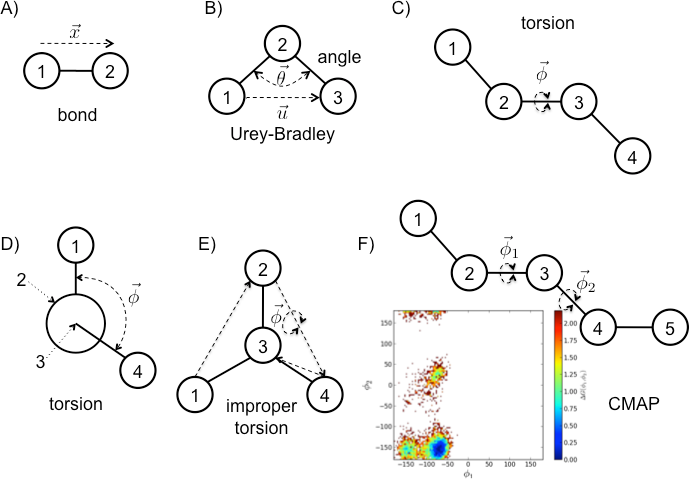
\includegraphics[width=6.5in,height=4.7in]{Parameters.png}
   \caption[Schematics shown for various parameters present in typical force
            fields.]
           {Schematics shown for various parameters present in typical force
            fields. A) is a bond parameter, B) shows the valence angle parameter
            and the Urey-Bradley parameter where $\vec{u}$ is the shown
            distance, C) depicts a torsion, D) depicts the same torsion using a
            Newman projection, E) depicts an improper torsion, and F) depicts
            two coupled torsions alongside a typical free energy map of two
            torsions that CMAP parameters attempt to fit to.}
   \label{fig1:Parameters}
\end{figure}

\subsection{The Amber Force Field}

The Amber force field is a popular family of force fields designed to treat
large biomolecules such as proteins, DNA, and RNA. This section will focus on
the functional form and implementation of the Amber force fields
\cite{Cornell_JAmChemSoc_1995_v117_p5179, Duan03, Hornak_Proteins_2006_v65_p712}
in the supporting Amber programs. \cite{Case_JComputChem_2005_v26_p1668}

\subsubsection{Functional Form}

The functional form of the Amber force fields is typically presented as in Eq.
\ref{eq1:AmberFF}, \cite{Cornell_JAmChemSoc_1995_v117_p5179} although this is an
incomplete specification. A more rigorous definition is presented in Eq.
\ref{eq1:AmberFF2}, taking into account the proper exclusion of non-bonded terms
between bonded atoms.

\begin{align}
   U(q) & = \sum _ {\text{bonds}} K_r ( r - r_{eq}) ^ 2 + \sum _ {\text{angles}}
          K_{\theta} ( \theta - \theta _ {eq} ) ^ 2 \nonumber \\
      & + \sum _ {\text{torsions}} \frac {V_n} 2 \left [ 1 + \cos (n \phi -
          \gamma) \right ] + \frac 1 2 \sum _ {i} \sum _ {j} \left [ \frac
          {A_{i,j}} {R_{i,j} ^ {12}} - \frac {B_{i,j}} {R_{i,j} ^ 6} + k_{elec}
          \frac {q_i q_j} {\epsilon R_{i, j}} \right ]
   \label{eq1:AmberFF}
\end{align}

\begin{align}
    & \sum _ {\text{bonds}} K_r ( r - r_{eq}) ^ 2 + \sum _ {\text{angles}} +
          K_{\theta} ( \theta - \theta _ {eq} ) ^ 2 \nonumber + \\
   U(q) = & \sum _ {\text{torsions}} \frac {V_n} 2 \left [ 1 + \cos (n \phi -
      \gamma) \right ] + \frac 1 2 \sum _ {i} \sum _ {j \in l_{1-4,i}} \left [
      \frac {A_{i,j}} {2.0 R_{i,j} ^ {12}} - \frac {B_{i,j}} {2.0 R_{i,j} ^ 6} +
      \frac {q_i q_j} {1.2 \epsilon R _{i,j}} \right ] +
      \label{eq1:AmberFF2} \\
    & \frac 1 2 \sum _ {i} \sum _ {j \notin l_{excl,i}} \left [ \frac {A_{i,j}}
      {R_{i,j} ^ {12}} - \frac {B_{i,j}} {R_{i,j} ^ 6} + k_{elec} \frac {q_i
      q_j} {\epsilon R_{i, j}} \right ] \nonumber
\end{align}

Amber employs a simple harmonic potential to model angles and bonds to
completely describe the interactions between atoms separated by one and two
bonds---\ie no electrostatic or Lennard-Jones potentials are calculated between
pairs of atoms connected by a bond or angle. Torsions are treated with a
truncated Fourier series expansion, typically using integral values for the
periodicity ($n$ in Eqs. \ref{eq1:AmberFF} and \ref{eq1:AmberFF2}). Therefore,
the sum over torsions in Eqs. \ref{eq1:AmberFF} and \ref{eq1:AmberFF2} is a sum
over all individual torsion terms for each distinct torsion. Improper torsions
are modeled the same way as `proper' torsions with only a single term designed
to maintain their planar geometry.

The non-bonded interactions are composed of a Lennard-Jones term (the third form
of Eq. \ref{eq1:LennardJones}) and electrostatic term calculated between all
atom pairs that are not excluded from the computation. The non-bonded exclusion
list---$l_{excl,i}$ for atom $i$ in Eq. \ref{eq1:AmberFF2}---is composed all
atoms separated by one, two, and three bonds (\ie that form bonds, angles, or
torsions with atom $i$). Finally, the LJ interactions between all atoms
separated by three bonds are scaled by $1/2$ and the electrostatic interactions
between those atom pairs are scaled by $1/1.2$. In Eq. \ref{eq1:AmberFF2},
$l_{1-4,i}$ represents the list of atoms related to atom $i$ like atoms 1 and
4 in Fig. \ref{fig1:Parameters}C.

\subsubsection{Implementation}

This section will describe how the Amber family of force fields is implemented
in the Amber program suite. It is important to note that the Amber force field
is not unique---there are many variants, each with a different name.
\cite{Cornell_JAmChemSoc_1995_v117_p5179, Wang_JComputChem_2000_v21_p1049,
Duan03, Wang_JComputChem_2004_v25_p1157, Hornak_Proteins_2006_v65_p712,
Zgarbova_JChemTheoryComput_2011_v7_p2886} All information necessary to fully
describe a molecular system with the Amber force field is contained in two
files---the parameter-topology file (\emph{prmtop}) and the coordinate file. The
prmtop file---fully described in Appendix \ref{appendixB}---contains all of the
information regarding the bonded network and the necessary parameters for
evaluating Eq. \ref{eq1:AmberFF2}. The coordinate file contains the Cartesian
coordinates and velocities for each atom in the system described by the prmtop
file.

The prmtop file is generated by the \emph{tleap} program by matching the
parameters from a database to the assigned `atom types' of the input structure.
Atom types are descriptors of individual atoms that specifies the properties and
typical chemical structure of bonds involving that atom. Each atom type, $i$,
has a predetermined set of atom parameters---an atomic mass, a LJ radius $r_i$,
and a LJ well-depth $\varepsilon_i$. The pairwise $R_{min,i,j}$ in Eq.
\ref{eq1:LennardJones} of atom types $i$ and $j$ is the sum $r_i + r_j$. The
combined well depth $\varepsilon_{i,j}$ is the geometric mean of the individual
well depths ($\sqrt {\varepsilon_i \varepsilon_j}$). These are the so-called
\emph{combining rules} employed by \emph{tleap} when parametrizing a molecule
with an Amber force field.

The Amber parameter databases store a list of all recognized atom types as well
as the bond, angle, and torsion parameters between the various bonded
arrangements of the available atom types. For instance, each pair of atom types
that could form a bond (\eg two aromatic carbons or an aromatic carbon and an
aromatic hydrogen) has an equilibrium bond length and bond force constant
associated with it. Also stored in these parameter databases are the equilibrium
angle displacements with corresponding force constants and torsion parameters
(periodicities, barrier heights, and phase shifts for each term of every
torsion).
